\documentclass{article}
% Change "article" to "report" to get rid of page number on title page
\usepackage{amsmath,amsfonts,amsthm,amssymb}
\usepackage{setspace}
\usepackage{Tabbing}
\usepackage{fancyhdr}
\usepackage{lastpage}
\usepackage{extramarks}
\usepackage{chngpage}
\usepackage{soul,color}
\usepackage{graphicx,float,wrapfig}
\usepackage{multirow,multicol,alltt}
\usepackage{enumerate}
% In case you need to adjust margins:
\topmargin=-0.45in      %
\evensidemargin=0in     %
\oddsidemargin=0in      %
\textwidth=6.5in        %
\textheight=9.0in       %
\headsep=0.25in         %

% Homework Specific Information
\newcommand{\hmwkTitle}{Representation:$(t_{ji},k_{jt})\Rightarrow(z_{ji},m_{ji})$}
\newcommand{\hmwkClass}{}
\newcommand{\hmwkAuthorName}{Donglai\ Wei}


% Setup the header and footer
\pagestyle{fancy}                                                       %
\lhead{\hmwkAuthorName}                                                 %
\rhead{\firstxmark}                                                     %
\lfoot{\lastxmark}                                                      %
\cfoot{}                                                                %
\rfoot{Page\ \thepage\ of\ \pageref{LastPage}}                          %
\renewcommand\headrulewidth{0.4pt}                                      %
\renewcommand\footrulewidth{0.4pt}                                      %

% This is used to trace down (pin point) problems
% in latexing a document:
%\tracingall

%%%%%%%%%%%%%%%%%%%%%%%%%%%%%%%%%%%%%%%%%%%%%%%%%%%%%%%%\begin{enumerate}

% Some tools
\newcommand{\enterProblemHeader}[1]{\nobreak\extramarks{#1}{#1 continued on next page\ldots}\nobreak%
                                    \nobreak\extramarks{#1 (continued)}{#1 continued on next page\ldots}\nobreak}%
\newcommand{\exitProblemHeader}[1]{\nobreak\extramarks{#1 (continued)}{#1 continued on next page\ldots}\nobreak%
                                   \nobreak\extramarks{#1}{}\nobreak}%

\newlength{\labelLength}
\newcommand{\labelAnswer}[2]
  {\settowidth{\labelLength}{#1}%
   \addtolength{\labelLength}{0.25in}%
   \changetext{}{-\labelLength}{}{}{}%
   \noindent\fbox{\begin{minipage}[c]{\columnwidth}#2\end{minipage}}%
   \marginpar{\fbox{#1}}%

   % We put the blank space above in order to make sure this
   % \marginpar gets correctly placed.
   \changetext{}{+\labelLength}{}{}{}}%

\setcounter{secnumdepth}{0}
\newcommand{\homeworkProblemName}{}%
\newcounter{homeworkProblemCounter}%
\newenvironment{homeworkProblem}[1][Problem \arabic{homeworkProblemCounter}]%
  {\stepcounter{homeworkProblemCounter}%
   \renewcommand{\homeworkProblemName}{#1}%
   \section{\homeworkProblemName}%
   \enterProblemHeader{\homeworkProblemName}}%
  {\exitProblemHeader{\homeworkProblemName}}%

\newcommand{\problemAnswer}[1]
  {\noindent\fbox{\begin{minipage}[c]{\columnwidth}#1\end{minipage}}}%

\newcommand{\problemLAnswer}[1]
  {\labelAnswer{\homeworkProblemName}{#1}}

\newcommand{\homeworkSectionName}{}%
\newlength{\homeworkSectionLabelLength}{}%
\newenvironment{homeworkSection}[1]%
  {% We put this space here to make sure we're not connected to the above.
   % Otherwise the changetext can do funny things to the other margin

   \renewcommand{\homeworkSectionName}{#1}%
   \settowidth{\homeworkSectionLabelLength}{\homeworkSectionName}%
   \addtolength{\homeworkSectionLabelLength}{0.25in}%
   \changetext{}{-\homeworkSectionLabelLength}{}{}{}%
   \subsection{\homeworkSectionName}%
   \enterProblemHeader{\homeworkProblemName\ [\homeworkSectionName]}}%
  {\enterProblemHeader{\homeworkProblemName}%

   % We put the blank space above in order to make sure this margin
   % change doesn't happen too soon (otherwise \sectionAnswer's can
   % get ugly about their \marginpar placement.
   \changetext{}{+\homeworkSectionLabelLength}{}{}{}}%

\newcommand{\sectionAnswer}[1]
  {% We put this space here to make sure we're disconnected from the previous
   % passage

   \noindent\fbox{\begin{minipage}[c]{\columnwidth}#1\end{minipage}}%
   \enterProblemHeader{\homeworkProblemName}\exitProblemHeader{\homeworkProblemName}%
   \marginpar{\fbox{\homeworkSectionName}}%

   % We put the blank space above in order to make sure this
   % \marginpar gets correctly placed.
   }%

%%%%%%%%%%%%%%%%%%%%%%%%%%%%%%%%%%%%%%%%%%%%%%%%%%%%%%%%%%%%%



%%%%%%%%%%%%%%%%%%%%%%%%%%%%%%%%%%%%%%%%%%%%%%%%%%%%%%%%%%%%%
% Make title
\title{\vspace{0.3in}\textmd{\textbf{\hmwkTitle}}}
\date{2011.4.28}
\author{\textbf{\hmwkAuthorName}}
%%%%%%%%%%%%%%%%%%%%%%%%%%%%%%%%%%%%%%%%%%%%%%%%%%%%%%%%%%%%%

\begin{document}
\begin{spacing}{1.1}
\maketitle
\section{0.Notation}
$t_{ji}$: table assignment of Customer i in restaurant j\\
$k_{jt}$: dish assignment of Table t in restaurant j \\
{\bf \large $l_{t_{ji}}$: the i th customer in restaurant j is sitting at the l lth table serving dish k }\\
$n^{l}_{jtk}$: number of customers in restaurant j sitting at table t, which is the l lth table serving dish k \\
$m_{jk}$: number of tables in restaurant j serving dish k.\\
{\bf . means marginalization}\\
$m_{.k}$: number of tables in dish k\\
$m_{j.}$: number of tables in Restaurant j\\
$n_{jt.}$: number of customers in Restaurant j table t\\
$n_{j..}$: number of tables in Restaurant j\\
$n_{..k}$: number of customers in dish k\\
$n_{..k}^{w}$ number of tables in dish k with word w\\
\section{1.CRF $(t_{ji},k_{jt})$}
$P(x_{ji},t_{ji},k_{jt}|\alpha,\gamma,\lambda)\\
=(table\ term)\displaystyle \Pi_{j=1}^{J} \{\frac{\Gamma(\alpha)}{\Gamma(n_{j..}+\alpha)}[\displaystyle \Pi_{t=1}^{m_{j.}}\Gamma(n_{jt.})] \alpha^{m_{j.}}\} \\
(dish\ term) \frac{\Gamma(\gamma)\displaystyle \Pi_{k=1}^{K}\Gamma(m_{.k})}{\Gamma(m_{..}+\gamma)}\displaystyle \Pi_{k=1}^{K} [\frac{\displaystyle \Pi_{w=1}^{W}\Gamma(\lambda_{0}+n_{..k}^{w})}{\Gamma(n_{..k}+W\lambda_{0})}
\frac{\Gamma(W\lambda_{0})}{\Gamma(\lambda_{0})^{W}}]\gamma^{K}\\
=C\times\displaystyle \Pi_{j=1}^{J} \displaystyle \Pi_{t=1}^{m_{j.}}\Gamma(n_{jt.}) \\
=C\times\displaystyle \Pi_{j=1}^{J} \displaystyle \Pi_{k=1}^{K}[\displaystyle \Pi_{l=1}^{m_{jk}}\Gamma(n^{l}_{j.k})] \\$
\section{2.CRF $(z_{ji},m_{jk})$}
Notice that $(t_{ji},k_{jt})=(z_{ji},l_{t_{ji}})$
\\Below, we are going to have a more compact assignment:sum over $l_{t_{ji}}\rightarrow \vec n_{j.k}\rightarrow m_{jk}$\\
$P(z_{ji},m_{jk}|\alpha,\gamma,\lambda)\\
=\displaystyle \sum_{partition} P(x_{ji},t_{ji},k_{jt}|\alpha,\gamma,\lambda)\\
=C\times\displaystyle \Pi_{j=1}^{J} \displaystyle \Pi_{k=1}^{K}\{\displaystyle \sum^{\sim}_{\vec n^{l}_{j.k}}[\left( \begin{array}{ccc} &n_{j.k} &\\n^{1}_{jk.}&...&n^{l}_{jk.} \end{array} \right)\displaystyle \Pi_{l=1}^{m_{jk}}\Gamma(n^{l}_{j.k})]\} \\
=C\times\displaystyle \Pi_{j=1}^{J} \displaystyle \Pi_{k=1}^{K}\left[ \begin{array}{c} n_{j.k} \\m_{jk} \end{array} \right] \\$
($\displaystyle \sum^{\sim}_{\vec n^{l}_{j.k}$:with constriants that $\displaystyle \sum \vec n^{l}_{j.k}=n_{j.k}$)\\
\begin{enumerate}
 \item Given $\vec n^{l}_{j.k}$, we sum over $l_{t_{ji}}$ configuration:\\
We get the factor $\left( \begin{array}{ccc} &n_{j.k} &\\n^{1}_{jk.}&...&n^{l}_{jk.} \end{array} \right)$
(number of combination to assign $n_{j.k}$ elements to $m_{jk}$ identifiable groups with size $\vec n^{l}_{j.k}$)
\item Given $m_{jk}$, we sum over $\vec n^{l}_{j.k}$\\
Then $\displaystyle \sum^{\sim}_{\vec n^{l}_{j.k}}\left( \begin{array}{ccc} &n_{j.k} &\\n^{1}_{jk.}&...&n^{l}_{jk.} \end{array} \right) [\displaystyle \Pi_{l=1}^{m_{jk}}\Gamma(n^{l}_{j.k})]$
exactly counts the number of permutations of $n_{j.k}$ elements with $m_{jk}$ disjoint cycles.
\end{enumerate}
\section{3.Will it solve the problem?}
\begin{enumerate}
 \item Suppose in the previous $(t_{ji},k_{jt})$ representation, $m_{jk}=\{0,1\}$, then:(modify s.t.$\Gamma(0)=1$)\\
$P(x_{ji},t_{ji},k_{jt}|\alpha,\gamma,\lambda)=C\times\displaystyle \Pi_{j=1}^{J} \displaystyle \Pi_{k=1}^{K}\Gamma(n_{j.k})\\$
$P(z_{ji},m_{jk}|\alpha,\gamma,\lambda)=C\times\displaystyle \Pi_{j=1}^{J} \displaystyle \Pi_{k=1}^{K}\left[ \begin{array}{c}
n_{j.k} \\
m_{jk} \end{array} \right] \\$
 \item Similar size:\\$ \Gamma(n_{j.k})<max(\left[ \begin{array}{c} n_{j.k} \\. \end{array} \right])=\left[ \begin{array}{c} n_{j.k} \\ * \end{array} \right]<\Gamma(n_{j.k}+1)$
 \item Penalty for splitting the table into 2:\\
For CRF($t_{ji},k_{jt}$):$\Delta(1\rightarrow2)=log\Gamma(n)-2log\Gamma(\frac{n}{2})\approx nlog(n)-2(\frac{n}{2})log(\frac{n}{2})=nlog(2)$\\
For CRF($z_{ji},m_{jk}$):$\Delta(1\rightarrow2)= log(\left[ \begin{array}{c} n \\ * \end{array} \right])-2log(\left[ \begin{array}{c} \frac{n}{2} \\ * \end{array} \right])$
\\There is no simple asymptotic approximation, but we can plot it numerically\\
We can see from the picture below, the penalty for splitting the table into 2 are similar.
\begin{center}
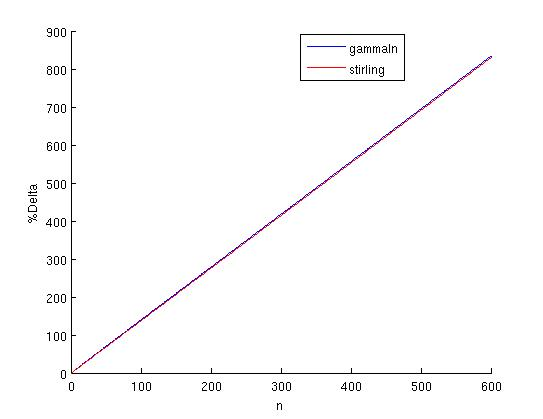
\includegraphics[width=5in,height=3in]{com.jpg} 
\end{center}
\end{enumerate}
{\bf Conclusion:}\\
\begin{enumerate}
 \item $\left[ \begin{array}{c} n_{j.k} \\ * \end{array} \right] $behaves similarly to $\Gamma(n_{j.k})$
 \item If the likelihood term is hard to improve, the restaurant still prefers one "dish" configuration
which has more partitions.
\item However, the degenate configuration now is sevaral tables serving the same dish instead of one big table 
serving that dish alone before.
\end{enumerate}

\end{enumerate}
\end{spacing}
\end{document}

%%%%%%%%%%%%%%%%%%%%%%%%%%%%%%%%%%%%%%%%%%%%%%%%%%%%%%%%%%%%%
